\documentclass[mathNotesPreamble]{subfiles}
\begin{document}
%\relscale{1.4}
\section{5.3: Fundamental Theorem of Calculus}
\begin{defn*}[Area Function]
  Let $f$ be a continuous function, for $t\geq a$. The \textbf{area function for $f$ with left endpoint $a$ is}
    \[A(x)=\int_a^x f(t)\,dt\]
  where $x\geq a$. The area function gives the net area of the region bounded by the graph of $f$ and the $t$-axis on the interval $\sbrkt{a,x}$.
\end{defn*}
\begin{ex*}
  The graph of $f$ is shown in the figure. Let $A(x)=\int_0^x f(t)\,dt$ and $F(x)=\int_2^x f(t)\,dt$ be two area functions for $f$. Evaluate the following area functions:
\end{ex*}

  \hfill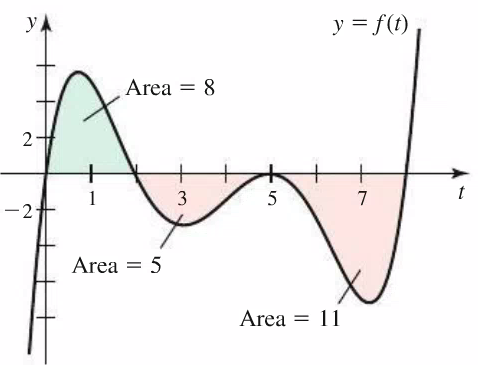
\includegraphics[width=0.5\linewidth]{images/briggs_05_03/q14.png}\hfill\mbox{} 

\begin{tasks}[after-item-skip=\stretch{1}](4)
  \task $A(2)$
  \task $F(5)$
  \task $A(0)$
  \task $F(8)$
  \task $A(8)$
  \task $A(5)$
  \task $F(2)$
\end{tasks}
\vspace*{\stretch{1}}
\pagebreak

\begin{ex*}
  Let $g(x)=\int_0^x f(t)\,dt$, where $f$ is the function whose graph is shown.
\end{ex*}
\noindent
\begin{minipage}[t]{0.55\linewidth}
  \begin{tasks}[after-item-skip=35pt](1)
    \task Evaluate $g(x)$ for $x=0,1,2,3,4,5$ and $6$.
    \task Estimate $g(7)$.
    \task Where does $g$ have a maximum value? Where does it have a minimum value?
  \end{tasks}
\end{minipage}
\begin{minipage}[t]{0.45\linewidth}\mbox{}
  \vspace*{-0.25\baselineskip}
  \begin{flushright}
    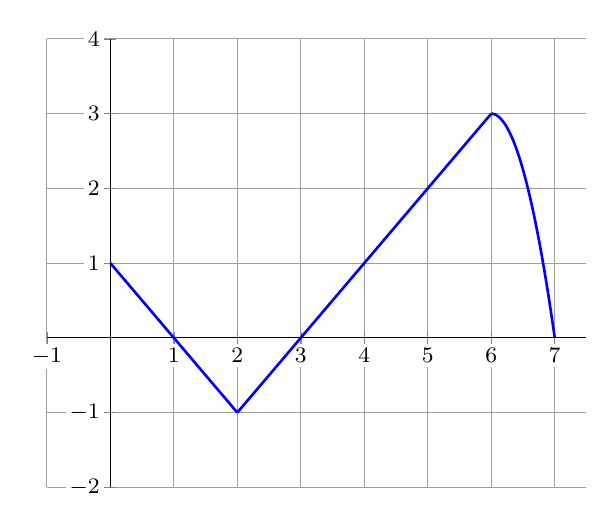
\begin{tikzpicture}
      \begin{axis}[
        grid=both,
        grid style={line width=0.35pt, draw=gray!75},
        axis lines=center,
        axis line style={-},
        xmin=-1, xmax=7.5,
        ymin=-2, ymax=4,
        xtick={-6,-5,...,7},
        ytick={-6,-5,...,6},
        ticklabel style={font=\footnotesize,inner sep=1.5pt,fill=white,opacity=1.0, text opacity=1},
        every axis plot/.append style={line width=0.95pt, color=blue, samples=100}
        ]
        \addplot[-] expression[domain=0:2]{1-x};
        \addplot[-] expression[domain=2:6]{x-3};
        \addplot[-] expression[domain=6:7]{-3*x^2+36*x-105};
      \end{axis}
    \end{tikzpicture}
    \hspace*{0pt}
  \end{flushright}
\end{minipage}
\vspace*{\stretch{1}}
\begin{ex*}
  For the area function $A(x)=\int_a^x f(t)\,dt$, graph the area function and then verify that $A'(x)=f(x)$.
\end{ex*}
\begin{tasks}[after-item-skip=\stretch{1}](1)
  \task $f(t)=10,\ a=4$
  \task $f(t)=2,\ a=-3$
\end{tasks}
\vspace*{\stretch{1}}
\pagebreak

\begin{tasks}[after-item-skip=\stretch{1}, resume](1)
  \task $f(t)=2t+5,\ a=0$
  \task $f(t)=4t+2,\ a=0$
\end{tasks}
\vspace*{\stretch{1}}

\begin{ex*}
  Let $f(x)=c$, where $c$ is a positive constant. Explain why an area function of $f$ is an increasing function.
\end{ex*}
\vspace*{\stretch{1}}

\begin{ex*}
  The linear function $f(x)=3-x$ is decreasing on the interval $\sbrkt{0,3}$. Is its area function for $f$ (with left endpoint 0) increasing or decreasing on the interval $\sbrkt{0,3}$?
\end{ex*}
\vspace*{\stretch{1}}
\pagebreak

\noindent
\fbox{\parbox{0.9875\linewidth}{
  \textbf{Theorem 5.3 (Part I) Fundamental Theorem of Calculus}

  \hspace*{10pt} 
  \parbox{0.9\linewidth}{
  If $f$ is continuous on $\sbrkt{a,b}$, then the area function
    \[A(x)=\int_a^x f(t)\,dt,\quad \textnormal{ for } a\leq x\leq b,\]
  is continuous on $\sbrkt{a,b}$ and differentiable on $\parens{a,b}$. The area function satisfies $A'(x)=f(x)$. Equivalently,
    \[A'(x)=\frac{d}{dx}\int_a^x f(t)\,dt=f(x).\]
}}}

\begin{ex*}
  For the following functions, find the derivatives
\end{ex*}
\begin{tasks}[after-item-skip=\stretch{1}](2)
  \task $g(x)=\ds\int_0^x \sqrt{1-2t}\,dt$
  \task $g(x)=\ds\int_3^x e^{t^2-t}\,dt$
  \task $g(y)=\ds\int_2^y t^2\sin(t)\,dt$
  \task $y=\ds\int_x^2 \cos(t^2)\,dt$
\end{tasks}
\vspace*{\stretch{1}}
\pagebreak

\begin{tasks}[after-item-skip=\stretch{1}, resume](2)
  \task $y=\ds\int_1^{\cos(x)} \parens{t+\sin(t)}\,dt$
  \task $y=\ds\int_{-3}^{3x^4} \frac{t}{t^2-4t}\,dt$
  \task $y=\ds\int_1^{e^x} \ln(t)\,dt$
  \task $y=\ds\int_0^{x^4} \cos^2(\theta)\,d\theta$
  \task $y=\ds\int_{\tan(x)}^0 \frac{dt}{1+t^2}$
  \task $y=\ds\int_{\sin(x)}^1 \sqrt{1+t^2}\,dt$
\end{tasks}
\vspace*{\stretch{1}}
\pagebreak

\noindent
\fbox{\parbox{0.9875\linewidth}{
  \textbf{Theorem 5.3 (Part II) Fundamental Theorem of Calculus}
  
  If $f$ is continuous on $\sbrkt{a,b}$ and $F$ is any antiderivative of $f$ on $\sbrkt{a,b}$, then
    \[\left.\int_a^b f(x)\,dx=F(b)-F(a)=F(x)\right|_a^b\]
}}

\begin{ex*}
  Evaluate the following integrals using graphs and the Fundamental Theorem of Calculus.
\end{ex*}
\begin{tasks}(2)
  \task $\ds\int_3^7 6\,du$
  \task $\ds\int_{-2}^4 x\,dx$
\end{tasks}
\vspace*{\stretch{1}}

\begin{ex*}
  Evaluate the following integrals
\end{ex*}
\begin{tasks}[after-item-skip=\stretch{1}](2)
  \task $\ds\int_{-1}^3 x^2\,dx$
  \task $\ds\int_0^\pi \parens{1+\cos(x)}\,dx$
  \task $\ds\int_{-5}^5 e\,dx$
  \task $\ds\int_0^{\pi/4} \sec\theta\tan\theta\,d\theta$
\end{tasks}
\vspace*{\stretch{1}}
\pagebreak

\begin{ex*}
  Evaluate the following integrals using the Fundamental Theorem of Calculus
\end{ex*}
\noindent
\begin{minipage}[t]{0.5\linewidth}\mbox{}%

  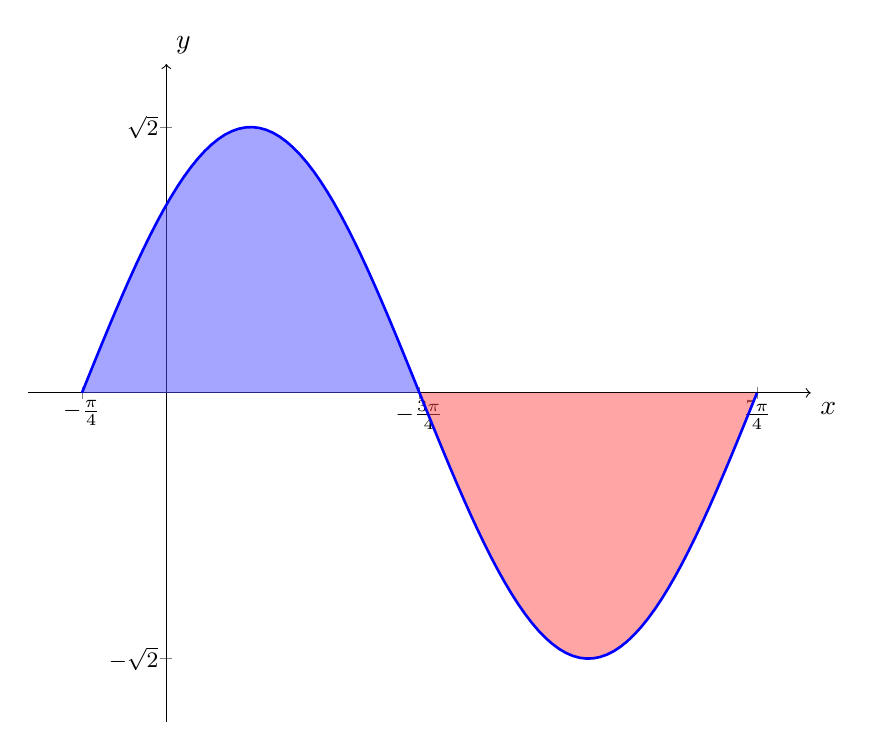
\begin{tikzpicture}
    \begin{axis}[
      axis lines=center,
      axis line style={->},
      xmin=-pi/4-0.5, xmax=7*pi/4+0.5,
      ymin=-1.75, ymax=1.75,
      xtick={-0.785398163,2.35619449,5.497787144},
      xticklabels={$-\frac{\pi}{4}$, $-\frac{3\pi}{4}$,$\frac{7\pi}{4}$},
      ytick={-1.414,1.414},
      yticklabels={$-\sqrt2$, $\sqrt2$},
      ticklabel style={font=\footnotesize,inner sep=0.5pt,fill=white,opacity=1.0, text opacity=1},
      width=0.95\linewidth,
      xlabel=$x$, xlabel style={at={(ticklabel* cs:1)},anchor=north west},
      ylabel=$y$, ylabel style={at={(ticklabel* cs:1)},anchor=south west},
      every axis plot/.append style={line width=0.95pt, color=blue, samples=100}
      ]
      \def\f(#1){sin(180*(#1)/pi)+cos(180*(#1)/pi)}
      
      \fill [blue!70, opacity=0.5, domain=-pi/4:3*pi/4, variable=\x]
        (-pi/4, 0)-- plot ({\x}, {\f(\x)})-- (3*pi/4, 0)-- cycle;
      \fill [red!70, opacity=0.5, domain=3*pi/4:7*pi/4, variable=\x]
        (3*pi/4, 0)-- plot ({\x}, {\f(\x)})-- (7*pi/4, 0)-- cycle;
      \addplot[-] expression[domain=-pi/4:7*pi/4]{\f(x)};
      \end{axis}
  \end{tikzpicture}
\end{minipage}%
\begin{minipage}[t]{0.5\linewidth}\mbox{}%

  $\ds\int_{-\pi/4}^{7\pi/4} \parens{\sin(x)+\cos(x)}\,dx$
\end{minipage}

\begin{ex*}
  Evaluate $\ds\int_3^8 f'(t)\,dt$, where $f'$ is continuous on $\sbrkt{3,8}$, $f(3)=4$, and $f(8)=20$.
\end{ex*}
\vspace*{\stretch{1}}

\begin{ex*}
  Find $\ds\frac{d}{dt} \int_0^{t^4} \sqrt{u}\,du$ by evaluating the integral directly and then differentiating the result.
\end{ex*}
\vspace*{\stretch{1}}
\pagebreak

\begin{ex*}
  Find $\ds\frac{d}{dt} \int_0^{t^4} \sqrt{u}\,du$ by differentiating the integral directly.
\end{ex*}
\vspace*{\stretch{1}}

\begin{ex*}
  Find $\ds\frac{d}{d\theta} \int_0^{\tan(\theta)} \sec^2(y)\,dy$ by evaluating the integral directly and then differentiating the result.
\end{ex*}
\vspace*{\stretch{1}}

\begin{ex*}
  Find $\ds\frac{d}{d\theta} \int_0^{\tan(\theta)} \sec^2(y)\,dy$ by differentiating the integral directly.
\end{ex*}
\vspace*{\stretch{1}}
\pagebreak

\begin{ex*}
  Evaluate the following integrals:
\end{ex*}
\begin{tasks}[after-item-skip=\stretch{1}](2)
  \task $\ds\int_1^8 \sqrt[3]{x}\,dx$
  \task $\ds\int_{-2}^{-1} \frac{2}{x^2}\,dx$
  \task $\ds\int_0^2 x(2+x^5)\,dx$
  \task $\ds\int_9^4 \frac{1-\sqrt{u}}{\sqrt{u}}\,du$
\end{tasks}
\vspace*{\stretch{1}}
\pagebreak

\begin{tasks}[after-item-skip=\stretch{1}, resume](2)
  \task $\ds\int_0^2 \parens{y-1}\parens{2y+1}\,dy$
  \task $\ds\int_0^4 \parens{1+3y-y^2-\frac{y^3}{4}}\,dy$
  \task $\ds\int_0^1 \parens{x^e+e^x}\,dx$
  \task $\ds\int_0^3 \parens{2\sin(x)-e^x}\,dx$
\end{tasks}
\vspace*{\stretch{1}}
\pagebreak

\begin{tasks}[after-item-skip=\stretch{1}, resume](2)
  \task $\ds\int_{\frac{\pi}{2}}^0 \frac{1-\cos(2t)}{2}\,dt$
  \task $\ds\int_{\frac{1}{2}}^2 \parens{1-\frac{1}{x^2}}\,dx$
  \task $\ds\int_1^2 \parens{\frac{2}{s^2}-\frac{4}{s^3}}\,ds$
  \task $\ds\int_{\frac{1}{\sqrt{3}}}^{\sqrt{3}} \frac{8}{1+x^2}\,dx$
\end{tasks}
\vspace*{\stretch{1}}
\pagebreak

%\begin{ex*}
%  Evaluate the following definite integrals:
%\end{ex*}
\begin{tasks}[after-item-skip=\stretch{1}, resume](2)
  \task $\ds\int_0^5 \parens{x^2-9}\,dx$
  \task $\ds\int_{-2}^{2} 6x^5+4x^3+2x\,dx$
  \task $\ds\int_{-1}^2 x^3\,dx$
  \task $\ds\int_{\pi/6}^{2\pi} \cos(x)\,dx$
\end{tasks}
\vspace*{\stretch{1}}
\pagebreak
%TODO Rogue example that I don't know where else to place
%$\ds\int_1^2 \frac{4+u^2}{u^3}\,du$

\begin{ex*}
  Find the area of the region bounded by $y=\sqrt{x}$ between $x=1$ and $x=4$.
\end{ex*}
\vspace*{\stretch{1}}

\begin{ex*}
  Find the area of the region below the $x$-axis bounded by $y=x^4-16$.
\end{ex*}
\vspace*{\stretch{1}}

\begin{ex*}
  Find the area of the region bounded by $y=6\cos(x)$ between $x=-\pi/2$ and $x=\pi$.
\end{ex*}
\vspace*{\stretch{1}}
\pagebreak

\begin{ex*}
  Find the area of the region bounded by $f(x)=x(x+1)(x-2)$ and the $x$-axis on the interval $\sbrkt{-1,2}$.
\end{ex*}
\vspace*{\stretch{1}}

\begin{ex*}
  Find the total area between $y=3x^2-3$ and the $x$-axis on $-2\leq x\leq 2$.
\end{ex*}
\vspace*{\stretch{1}}

\begin{ex*}
  Find the total area between $y=x^3-3x^2+2x$ and the $x$ axis on the interval $0\leq x\leq 2$.
\end{ex*}
\vspace*{\stretch{1}}
\pagebreak
%TODO Comment out relscale
\end{document}
